\chapter{Растрові зображення}\label{cha:bitmap_image}

Растрові, зображення є «цифровими фотографіями», вони є найпоширенішою формою для представлення природних зображень та інших видів графіки, які багаті на деталі.
Растрові зображення - це те, як графіка зберігається у відеопам’яті комп’ютера.
Термін растрове зображення стосується того, як заданий шаблон бітів у пікселі відображається до певного кольору.
Попередній опис зображення можна розглядати як "рецепт приготування", як намалювати зображення, він містить геометричні примітиви, такі як лінії, криві та кола, що описують колір, а також відносний розмір, положення та форму елементів.
Коли підготовка зображення до відображення повинна бути перетворена у растрове зображення, цей процес називається растеризацією.

Растрові зображення набувають форми масиву, де значення кожного елемента, який називається елементом \textbf{піксельного(pixel) зображення}, відповідає кольору цієї частини зображення.
Де горизонтальна лінія на зображенні називається \textbf{лінією сканування(scan line)}.

Буква "а" може бути представлена в матриці 12x14, як показано на малюнку 3., значення в матриці відображають яскравість \textbf{пікселів} (елементів зображення).
Більші значення відповідають світлішим областям, тоді як нижчі значення темнішим.

\begin{figure}
    \label{fig:image4}
    \centering
    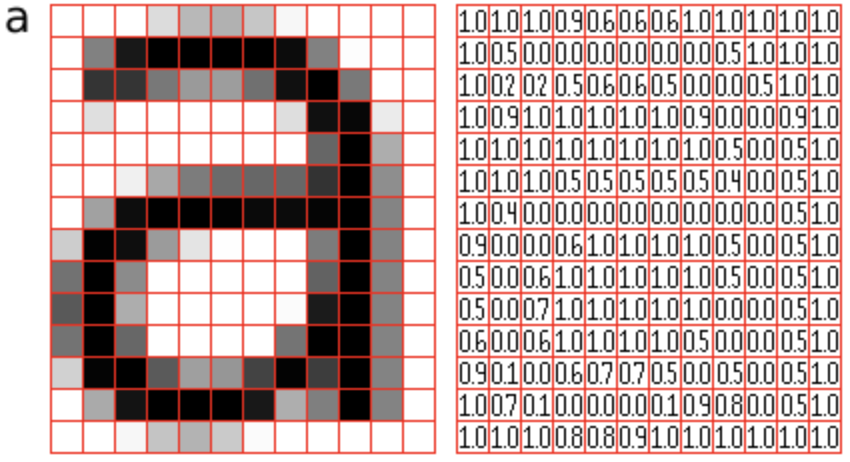
\includegraphics[scale=0.5]{image4.png}

    Рис. 4. Растеризована форма букви "а" збільшена в 16 разів за допомогою подвоєння пікселів
\end{figure}

\section{Растровий розмір}\label{sec:raster_sdimensions}
Кількість горизонтальних і вертикальних зразків у піксельній сітці називається \textbf{растровим розміром(raster dimension)}, вона визначається як ширина X висота.
